% This .tex file (and associated .cls) produces:
%       1) The Permission Statement
%       2) The Conference (location) Info information
%       3) The Copyright Line TSConIT
%       4) NO page numbers
%       5) NO headers and/or footers
%
% Using 'sig-alternate.cls' you have control, however, from within
% the source .tex file, over both the CopyrightYear
% (defaulted to 200X) and the ACM Copyright Data
% (defaulted to X-XXXXX-XX-X/XX/XX).
% e.g.
% \crdata{0-12345-67-8/90/12} will cause 0-12345-67-8/90/12 to appear in the copyright line.
%

% This .tex source is an example which *does* use
% the .bib file (from which the .bbl file % is produced).
% REMEMBER HOWEVER: After having produced the .bbl file,
% and prior to final submission, you *NEED* to 'insert'
% your .bbl file into your source .tex file so as to provide
% ONE 'self-contained' source file.
%
% refers to the cls file being used
\documentclass{sig-alternate-br}
\usepackage{float}
\usepackage{caption}
\usepackage{subcaption}
\usepackage{hyperref}
\usepackage{xcolor}
\usepackage{enumitem}
\usepackage{tabularx}

\usepackage[numbers]{natbib}
\setlength{\bibsep}{0.0pt}
\restylefloat{figure}
\restylefloat{table}
\begin{document}
\setcounter{page}{1}
\pagenumbering{arabic}
%
% --- Author Metadata here --- DO NOT REMOVE OR CHANGE 
\conferenceinfo{23$^{th}$ Twente Student Conference on IT}{June 22$^{st}$, 2015, Enschede, The Netherlands.}
\CopyrightYear{2015} % Allows default copyright year (200X) to be over-ridden - IF NEED BE.
%\crdata{0-12345-67-8/90/01}  % Allows default copyright data (0-89791-88-6/97/05) to be over-ridden - IF NEED BE.
% --- End of Author Metadata ---

\title{Small Data Center using Raspberry Pi 2 for Video Streaming}
% In Bachelor Referaat at University of Twente the use of a subtitle is discouraged.
 \subtitle{}


\numberofauthors{1} 
\author{ 
% You can go ahead and credit any number of authors here,
% e.g. one 'row of three' or two rows (consisting of one row of three
% and a second row of one, two or three).
%
% The command \alignauthor (no curly braces needed) should
% precede each author name, affiliation/snail-mail address and
% e-mail address. Additionally, tag each line of
% affiliation/address with \affaddr, and tag the
% e-mail address with \email.
%
% 1st. author
\alignauthor P.J.E. Velthuis\\
       \affaddr{University of Twente}\\
       \affaddr{P.O. Box 217, 7500AE Enschede}\\
       \affaddr{The Netherlands}\\
       \email{p.j.e.velthuis@student.utwente.nl}
% 2nd. author
\alignauthor 2nd Author\\
       \affaddr{2nd author's affiliation}\\
       \affaddr{1st line of address}\\
       \affaddr{2nd line of address}\\
       \email{2nd author's email address}
% 3rd. author
\alignauthor 3rd Author\\
       \affaddr{3rd author's affiliation}\\
       \affaddr{1st line of address}\\
       \affaddr{2nd line of address}\\
       \email{3rd author's email address}
}

%\additionalauthors{Additional authors: John Smith (The
%Th{\o}rv{\"a}ld Group, email: {\texttt{jsmith@affiliation.org}})
%and Julius P.~Kumquat (The Kumquat Consortium, email:
%{\texttt{jpkumquat@consortium.net}}).}
%\date{30 July 1999}


\maketitle
\begin{abstract}
Cloud computing is a IT trend  in which customers move computing and data away from computer and laptop into data centers. These data centers require a lot of power and cooling. Nowadays, approximately 30\% of the data coming from these centers is video streaming. The Raspberry Pi 2 is a low cost device that can be used in a cloud for video streaming. In this paper a further investigation in the Raspberry Pi 2 cloud is done. This research is a design research in which a design is made for a video streaming cloud consisting of Raspberry Pi's. In this research it turned out that the Raspberry Pi 2 has its hardware limits. The results is that it is not so useful inside a data center, but it is good for education purposes.  In this research it was possible to run different video streaming algorithms. The Raspberry Pi 2 turned out to be a great device for doing research into video streaming.
\end{abstract}

\keywords{Cloud computing, Raspberry Pi 2, RPi2,  micro data center, video streaming, load balancing}

\section{Introduction}
Today, most of us have data in the cloud. Despite the attention from the community, research and development of Cloud Computing services are still in its early days~\citep{tso:2013}. \newline
Cloud computing is a trend in IT that moves customers computing and data away from computer, and laptop into large data centers \citep{dikaiakos:2009}. In the future, most Internet users are expected to access Internet services over lightweight portable devices requiring a lot of network bandwidth \cite{dikaiakos:2009}. This bandwidth usage causes bottlenecks. To prevent these bottlenecks, data centers are built around the globe. These data centers can be greatly improved \cite{abrahamsson:2013,beloglazov:2010}. 
For example, these data centers require a lot of space and cooling. There are now new technologies such as the powerful ARM processor. Companies want to explore the possibilities of the Raspberry Pi 2 (RPi2), because of its ARM processor and the low price \cite{Pcextreme}. At the time of writing the RPi2 costs around 40 euro. The RPi2 is cheaper in price compared to a more expensive normal server. Some data centers offer some cloud computing using the Raspberry Pi 2 \cite{Pcextreme}. \newline
A RPi2 is a small computer and has a power usage between two and four Watt. In contrast, a normal server has a power usage between 75 and 250 Watt~\cite{Pcextreme,beloglazov2012energy}. The low power consumption of the RPi2 and its computing power could mean that it is better to use a RPi2 for specific small tasks that do not demand an entire server. For this reason, research is done on the performance of the RPi2 in a small data center. \newline
A Raspberry Pi cloud can be the small data center for the future \cite{tso:2013}. The RPi2 can be an ideal testbed for testing distributed software. 

In The Netherlands one million people use Netflix \cite{volkskrant}. Netflix is a popular video streaming service that provides HD movies. To achieve this Netflix makes use of a Content Distribution Network (CDN). Netflix makes use of MPEG-DASH, a protocol for streaming over HTTP \cite{martin:2013}. The problem is that Netflix is responsible for approximately 30 \% of the peak downstream traffic in the US \cite{Adhikari:2012}. The result was that the two main providers Comcast and  AT\&T were limiting the downstream traffic of Netflix. This caused a lot of criticism, to solve this a new law for net neutrality has been made \cite{net-neutrality}. \newline
In the Netherlands, video streaming services such as Youtube and Netflix have an increasing number of users. Nowadays, the data streaming problems are increasing, this makes it interesting to do more research in data centers with video streaming. Most of the existing research in computer science is performed on expensive large servers \cite{tso:2013}. It can be very useful to see if it is possible to do research on a small computer like a RPi2.

This paper investigates how useful the RPi2 is in a data center with video streaming. To come to a conclusion the performance of the RPi2 is evaluated by doing several benchmark tests. For this the main research question is: 
\begin{center}
How well does the RPi2 perform in small scale data centers with video streaming? 
\end{center}

To answer for the main question, several sub-questions are researched, which are:

\begin{enumerate}
	\item What are small scale data centers with video streaming and why are they used?
	\item Is the RPi2 usable for video streaming?
	\item How to fit the RPi2s into a data center considering cooling, space allocation and power?
	\item What setup does a RPi2 cloud with video streaming require?
	\item How is availability in a RPi2 cluster with video streaming affected by various load balancing techniques? 
\end{enumerate}

The five sub-questions are investigated in the next sections. Followed by a final section for conclusions and identified areas for future work.
The first two research question are a literature study into video streaming and cloud computing. The last three sub-questions go into the technical research that investigates the performance and possibility of RPi2s for cloud video streaming. This is done by building a small RPi2 cloud. 

\section{Research Methods}
In the research the  aim is to build a RPi2 cloud to measure the performance. This is achieved by building a RPi2 cloud and doing benchmark test on this cloud. This research uses the Design Science method proposed by Hevner~\cite{hevner:2007}. The method is used to make an architecture for a Raspberry Pi cloud. This design science method consists of three cycles:
\begin{figure}[H]
	\centering 
	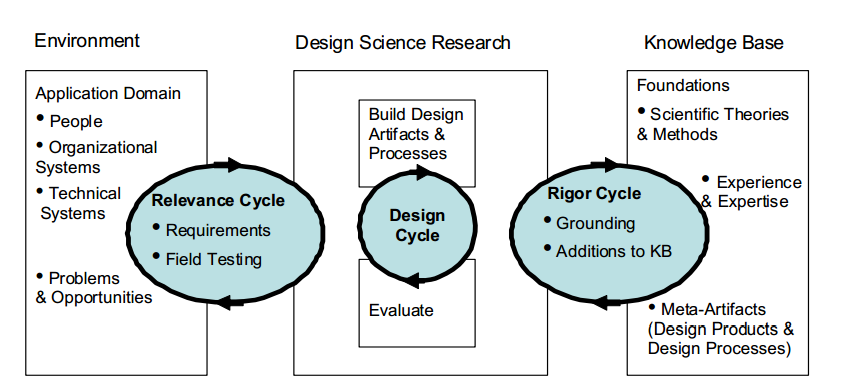
\includegraphics[width=0.4\textwidth]{Design_science.png}
	\caption{Design Science cycles \cite{hevner:2007}}
	\label{fig:design} %always place your label after your caption!
\end{figure}
\textbf{relevance cycle} Represents the interaction with the domain. Here the problems and opportunities are identified. The identification of these problems are done in the next section. \newline 
\textbf{design cycle} The most important cycle where the design is built. This is highlighted in section \ref{sec:setupex}. \newline
\textbf{rigor cycle} Represents the interaction with the scientific community. This information can be found in section \ref{sec:back} and \ref{sec:setupex}.



\section{Background}\label{sec:back}
\subsection{Small scale computing}
Small scale cloud computing is cloud computing with smaller computation amounts than normal \cite{cox:2014}. Most customers for cloud solutions buy the services instead of buying the hardware and having to set up the servers themselves. This service is called Infrastructure as a Service (IaaS). The elasticity of computing resources in the cloud is important to provide IaaS \cite{Miettinen:2010:EEM:1863103.1863107}. Many companies have their software running on virtual machines in data centers \cite{beloglazov:2010}. The advantage is that these virtual machines are scaled dynamically to the customers need. Using the cloud makes  management easier. 

Several cloud services have a huge network demand, this may cause data centers to be unreachable. Because of the privacy and reachability of a data center many companies have their own servers. These servers are not energy efficient. \newline
Netflix, a cloud service, is responsible for approximately 30\% of the peak downstream traffic in the US \cite{Adhikari:2012, computer-networking}. The data flowing through the network has different patterns. To improve this there are several data patterns possible, it can for example make a huge different in sending data in small bursts or in one large burst \cite{computer-networking}.

Power Usage Efficiency (PUE) is a important aspect in cloud computing \cite{beloglazov2012energy}. There are more lightweight portable devices coming \cite{Miettinen:2010:EEM:1863103.1863107}, these devices are energy efficient, but will demand more processes by data centers \cite{Miettinen:2010:EEM:1863103.1863107}. Nowadays, the data centers operate 12 to 20\% of the time, the other 80 \% of the time the servers inside are still using energy \cite{beloglazov2012energy, meisner2009powernap}. Therefore there is a need for Green Cloud Computing solutions that reduce the electrical power consumption and the environmental impact of data centers~\cite{beloglazov2012energy}. Microservers can be used to reduce the electricity consumption.

\subsection{Microserver}
Microservers are used in data centers \cite{microserver}. Microservers consume less electricity and have enough computer power for small tasks, therefore they can be used for high traffic usage tasks. Besides this they are small and are easier replaced compared to a normal server, by using them data centers can be more dynamic \cite{microserver}. The ability to add and remove microservers more easily can save a lot of energy. \newline
A microserver often has a different processor compared to a normal server. The processors are often microprocessors like ARM processors \cite{microserver}. There are three big processor companies in the world: ARM, Intel and AMD. The Intel and AMD processors are better at complex tasks, while the ARM processor is better at small tasks \cite{microserver}. In the data center of the future more dedicated microservers will be used, they are better at specialized tasks and are more energy efficient \cite{microserver}. 

\subsection{Video streaming}\label{sec:stream}
HTTP is used for video streaming, HTTP sends frames to the client and in the frames is the video stored \cite{computer-networking}. If the send rate is large enough the video will play without any delays, but if the send rate is too low then the video playback will alternate between periods of continuous playback and periods of freezing~\cite{computer-networking}. \newline 
To make video streaming possible the client will connect with video streaming service by its load balancer. The load balancer will then locate the videos. To show how the processes and operators operate with each other, the UML sequence diagram in figure \ref{fig:stream} is used \cite{Bernardi:2002:USD:584369.584376}. 
\begin{figure}[H]
	\centering 
	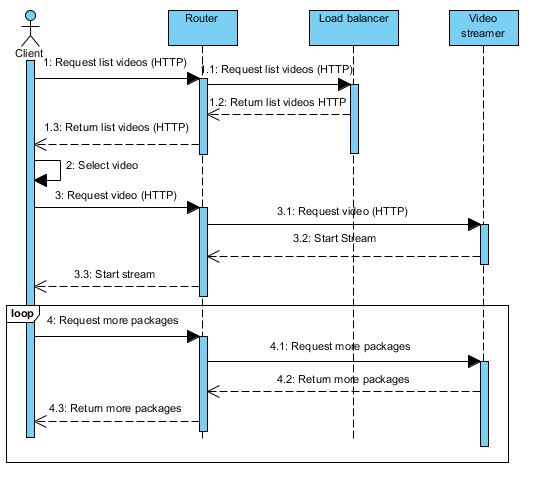
\includegraphics[width=0.4\textwidth]{VideoStreaming.jpg}
	\caption{Video stream}
	\label{fig:stream} %always place your label after your caption!
\end{figure}

In the diagram there is a loop for the video streaming, here the client will keep requesting more parts of the videos. Depending on the algorithm being used the amount of data requested by the client can fluctuate. For streaming a video HTTP streaming is often used. If the client receives too much data its buffer gets full. To prevent throwing data away the server then stops sending.

There is a important streaming technique called adaptive streaming \cite{computer-networking}. This streaming algorithm is often used for video on demand (VOD) \cite{computer-networking}. It improves the experience for the end-user by adapting the video quality dynamically to the viewers network condition \cite{ffmpeg}. This techniques takes into account the clients CPU possibility and its network possibilities. It delivers small sized chunks at multiple bitrates. This techniques is used for HTTP Live Streaming (HLS) \cite{jwplayer}. HLS makes use of RTMP streaming and HTTP. HLS codifies video in the H.264 format.\newline
There is another special kind of HTTP streaming called DASH (Dynamic Adaptive Streaming over HTTP)~\cite{computer-networking}. In DASH the video is encoded into several different versions. If the bandwidth is high, then the client selects chunks from a high-rate version and the other way around~\cite{computer-networking}. The possibility to switch between versions of different bitrates is in video streaming important for user experience. To make a smooth transition between these versions possible there are intermediate versions so that the client will see the change in video quality less suddenly. 

\subsection{Video streaming and load balancing}
For video streaming several load balancing techniques are used. To choose a technique the following aspects are taken into account performance, reliability and features. There can be a non-uniform demand for different movies. One solution to overcome this problem would be to replicate the most popular movies, but this is expensive in terms of storage space required for this. A dynamic replication can be used to solve the load demand~\cite{dan1996load}. Parts of a movie are moved to less used storage devices, so that these can stream the movie. The allocation of these movies only happens when there is a too high increase on one specific storage device. In this way load imbalances can be prevented \cite{dan1996load}. \newline
Load balancers are generally grouped in two layers. Layer 4, the transport layer and layer 7 the application layer \cite{computer-networking}. Layer 7 load balancers distribute requests based upon data in the application layer. Here below are two protocols and a language that is used:
\begin{enumerate}[topsep=0pt,itemsep=-1ex,partopsep=1ex,parsep=1ex]
	\item HTTP, is the hypertext transfer protocol. In section \ref{sec:stream} usages of this protocol are mentioned. A lot of video streaming services use HTTP streaming \cite{Adhikari:2012}.  
	\item RTMP is a real time messaging protocol ~\cite{rtmp}. It is developed for streaming data between a player and a server. It is encapsulated in HTTP to traverse firewalls. It gives more video player options compared to normal HTTP, thus giving the user a better experience. A disadvantage compared to normal HTTP is that it is sensitive for data spikes. These data spikes can result in a overload of the buffer which results in a empty buffer, this can lead to a stop in the video playing. 
	\item Synchronized Multimedia Integration Language (SMIL) describes multimedia presentations \cite{smil}. SMIL refers to media objects by URLs, allowing them to be shared between presentations and stored on different servers for load balancing. 
\end{enumerate}


\subsection{Video streaming in a data center}

Users want on demand video streaming, because they do not want to store the data themselves, and want a wide choice of different videos on demand. Netflix is a on demand video streaming service that makes HD movies watching possible. For this Netflix uses a content distribution network (CDN). Netflix uses amazon its AWS, simpleDB, S3 and Cassandra for file storage \cite{Adhikari:2012}. Netflix makes use of MPEG-DASH, a protocol that makes streaming over HTTP possible. To make this possible Netflix does several things in the cloud. 

 \begin{enumerate}[topsep=0pt,itemsep=-1ex,partopsep=1ex,parsep=1ex]
 	\item Content ingestion, this means that Netflix receives the studio master version of the movies and uploads these to the cloud. 
 	\item Content processing, this means that in the cloud many different formats are created for each movie.
 	\item Uploading different versions to the CDN,	this means that all the versions that have been made are distributed over the CDN.
 \end{enumerate}
Netflix ~\cite{Adhikari:2012}




\subsubsection{Video stream CDN}
A CDN uses small data centers, because users want their data as nearby as possible  In this way the latency is decreased and there is a shorter connection distance, this gives the user faster load times. Video streamer Netflix has  its own CDN \cite{netflix}. Reasons for having an own CDN is that the load balancing can be improved. The CDN that Netflix has created is called Open Connect. Netflix uses high performance HTTP delivery to get the content to the users. Data going over the network can be decreased and videos get faster to users with an own CDN, because video stream algorithms are better analyzed. 

\section{Related work}

There have been several cloud projects with the Raspberry Pi. \newline
One was the supercomputer built by Southampton~\cite{cox:2014}. Here a cluster was built with 64 raspberry Pi's. A Message Passing interface was used to communicate between the Raspberry Pi's. The research was done in order to see what the performance of a low-power high performance cluster was. \newline
The project of the university of Glasgow~\cite{tso:2013}. This data center has 56 Raspberry Pi's. It was built for research and education purposes for a cloud data center. Hadoop was tested on their servers. \newline
Another project called the Beowulf cluster~\cite{beowolf-setup}. This project was created for a PhD assignment. This cluster was built for collaboratively processing sensor data.  A Beowulf cluster is simply a collection of identical, commodity computer hardware based systems~\cite{beowolf-setup}. The big advantage of the Raspberry Pi in this project was that it was cheap and it does not need a cluster administrator to check everything that was being done. 

For Video streaming there are several projects. These projects are often done by service providers. \newline
Netflix works together with NGINX on Netflix his project Open Connect. With this cooperation they want to give  users the best video watching experience. This project wants to improve the load balancing for video streaming over the whole network. \newline
Another service is WOWZA \cite{wowza}. WOWZA provides video streaming for a lot of companies and universities. WOWZA has done several projects for video streaming and has built with the University of Maine a content management system for their online videos. \newline 
One mayor video stream service is of course Youtube \cite{youtube}. Youtube was once started as a project with the aim to remove the technical barriers to share videos online. Nowadays Youtube is still working hard on optimizing their video streaming service. Youtube has a online API, so developers can join in and start their own projects. Youtube has its own projects for example helping mobile gamers stream their video and helping with live streaming.

\section{System description}\label{sec:system}

\begin{figure}[H]
	\centering 
	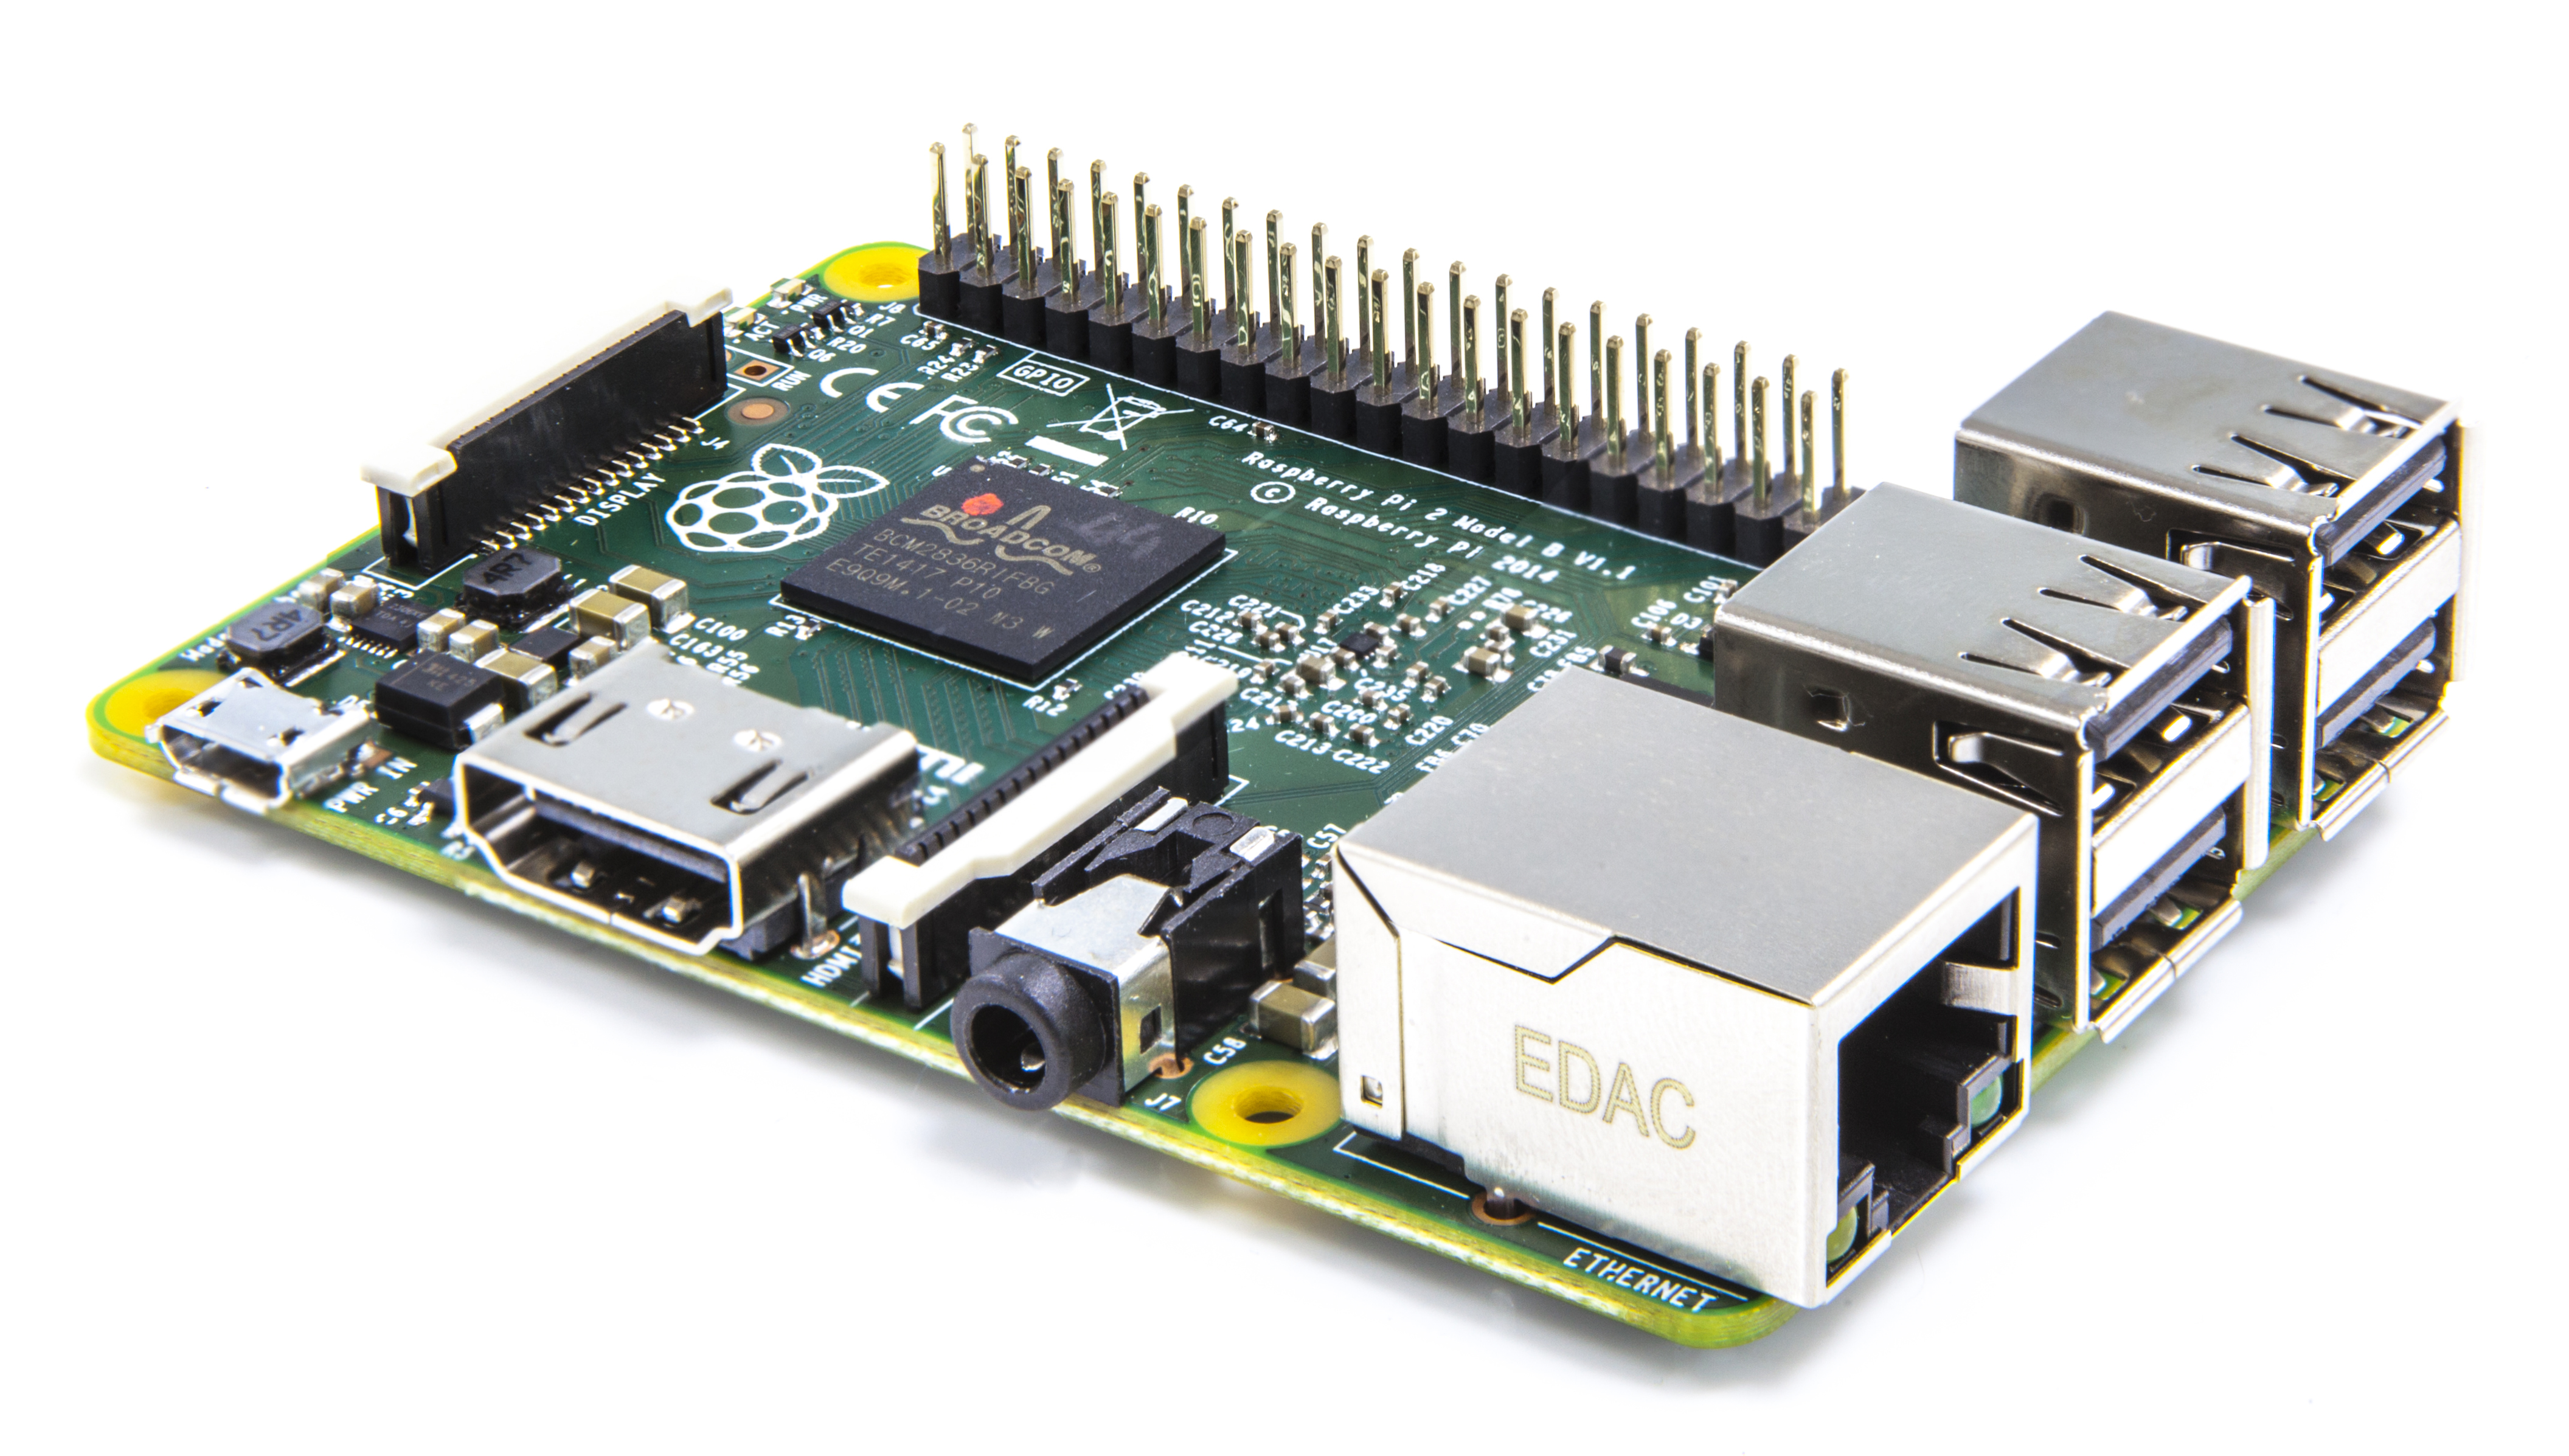
\includegraphics[width=0.4\textwidth]{Pi2ModB1GB_-comp.jpeg}
	\caption{Raspberry Pi 2 model B \cite{raspberry-pi}}
	\label{fig:raspberry} %always place your label after your caption!
\end{figure}
\begin{table}[H]
	\centering \caption{Specifications \cite{raspberry-pi}}
	\begin{tabular}{|c|c|} \hline
		Ethernet & 100 Mbps \\ \hline
		USB & 4 x USB 2.0 \\ \hline
		Video out & HDMI 1.4 \\ \hline
		Audio & 2 x analog \\ \hline
		CPU & 900MHz quad-core ARM Cortex-A7 \\ \hline
		card slot & Micro SD  \\ \hline
	\end{tabular}
	\label{tab:Specificaties}
\end{table}
The RPi2 only consumes 3 Watt, because of this it does not need active cooling. The RPi2 has a limited ethernet interface of only 100 Mbps. The network cable offers room for analyzing the video stream. The USB 2.0 is used to share the data from a external harddisk to a user. A external Seagate harddisk demands 10 Watt when it is actively streaming videos and when it is standby it has a consumption of 0.1  Watt.

This research makes use of three Raspberry Pi's one router and one switch. All these Pi's need power, therefore there is a power supply and 3 micro USB cables. There are three sd cards needed for the Operating System, and other software, to make the RPi2 work. A cost structure for this can be found in the appendix section~\nameref{sec:cost}.

For some benchmark tests a laptop is plugged in, so that several tests can be done from the laptop.


\section{Setup \& Experiment}\label{sec:setupex}


\subsection{Experiment approach}
This setup is built by following the information in the GitHub link in section \ref{sec:software}, that can be found in the appendix. More details about the setup can be found in section \ref{sec:setup}. \newline 
A RPi2 is used for video streaming with load balancing. For the experiment we need a Raspberry Pi 2 that can make use of the Internet. This is because a RPi2 is used as a webserver to make video streaming possible. It has a VPN to make it possible to put video's on the RPi2. 
A cluster with one RPi2 as a load balancer and the other two as a video stream Pi is built. If such a cluster is made tests can be done and improvements can be made. For example streaming tests with different quality videos and load balancing. The test are found in section \ref{sec:test}. Below the setup design and legend for the RPi2 are given:
\begin{enumerate}[topsep=0pt,itemsep=-1ex,partopsep=1ex,parsep=1ex] 
	\item The client who wants to get the video. 
	\item The router who redirects the client to the load balancer. The router will also have the video streamers in this network. If there are to much Raspberry Pi's in a network to connect to a single router a switch can be placed between them. 
	\item The load balancer who redirects the client to the right video streamer.
	\item The video streamer who streams the video to the client.
	\item The video streamer who streams the video to the client.
\end{enumerate}
For the research number three to five are Raspberry Pi's.
\begin{figure}[H]
	\centering 
	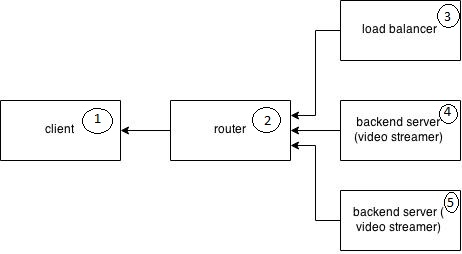
\includegraphics[width=0.5\textwidth]{raspsetup.jpg}
	\caption{Raspberry Setup}
	\label{fig:setup} %always place your label after your caption!
\end{figure}


\subsection{RPi2 inside a data center}

In this part the research focuses on the possibilities of the RPi2 in a data center. \newline
It is possible to fit a lot of RPi2s inside a data center. PCextreme has placed 500 Pi's inside a single data rack \cite{Pcextreme}. For this special designed boards are needed. With a special board RPi2 can be rebooted and turned off from a distance \cite{Pcextreme}. By having a microserver like a RPi2 in a data center the hardware can be owned by only the customer, because its better payable than a normal server. In a data center there are the advantages of the high speed Internet. By owning the hardware the customer will have more control over the data in the privacy and reliability aspect.\newline In this research there are 3 Pi's and these fit easily inside the rack. The cooling of the data rack is sufficient for all these RPi2s. The power consumption of the RPi2 is low as seen in table \ref{tab:cpu}. The RPi2 is easy to replace and it can easily be turned on and off, this makes it suitable inside a server rack. A problem that will exist with the RPi2 inside the data center is that every time a Pi's have troubles a help team inside the data center has to fix this for the customer. 

In this project a cluster of RPi2s is built to test its possibilities. The setup for this project is displayed below:
\begin{figure}[H]
	\centering 
	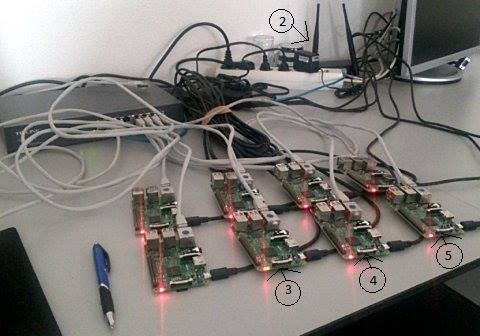
\includegraphics[width=0.45\textwidth]{setup.jpg}
	\caption{Project Setup}
	\label{fig:projectsetup} %always place your label after your caption!
\end{figure}
The numbers in front in figure \ref{fig:projectsetup} point to the RPi2s, these numbers correspond with the numbers in figure \ref{fig:setup}. The number in the back shows the little router that is behind the power supply. In this picture there is a extra switch to connect all the Raspberry Pi's. \newline 
This setup can be placed inside of a data center. The switch and the router will then be removed and the rest will be fit into the server rack. 

To verify that a Pi2 can operate inside a data center some tests have been done. For these tests a multimeter has been used. The Elro M990 multimeter has been used. The program sysbench has been used to run several CPU tests for the RPi2 its four cores. This is a benchmark test to get a quick impression about the performance of the system. The ampère and volt is measured with the multimeter during the test. the This gave the following results:
\begin{table}[H]
	\centering \caption{CPU test}
	\begin{tabular}{|c|c|c|c|} \hline
		Test & Ampère (A) & Volt (V) & Watt (W)\\ \hline
		CPU 1 core & 0.340 & 4.84  & 1.65\\ \hline
		CPU 2 cores & 0.365 & 4.79 & 1.75\\ \hline
		CPU 3 cores & 0.392 & 4.77 & 1.87 \\ \hline
		CPU 4 cores & 0.415 & 4.78 & 1.99 \\ \hline
		Memory test & 0.440 & 4.79 & 2.11 \\ \hline
		Storage read & 0.442 & 4.77 & 2.11\\ \hline
		Storage write & 0.395 & 4.77 & 1.89 \\ \hline
		Idle & 0.315 & 4.78 & 1.51 \\ \hline
	\end{tabular}
	\label{tab:cpu}
\end{table}
A normal server needs about 500 W \cite{meisner2009powernap}. The RPi2 has a consumption in this test of about 2.1 W see table \ref{tab:cpu}. With a simple calculation is seen that 500/2.1=238 Pi's are possible instead of one server. The idle temperature is only 1.5 W, while normal severs still need 60 \% of the power \cite{meisner2009powernap}. By using these small modular systems the power consumption inside a data center can be improved. The space usage is not optimal, because the RPi2 has a micro USB cable  in one corner and an ethernet cable in the other as can be seen in figure \ref{fig:raspberry}. 
Improvements can be made by letting the power go over the ethernet by using a Power over Ethernet equipment. Another solution can be by making a motherboard on which  Raspberry Pi modules can be plugged instead of a whole device, This is future work. \newline
There is a Temperature test done by running the same tests and measuring the temperature by using a self written script. The temperature is measured on the CPU. The room temperature during this test was around 23 degrees Celsius. 

\begin{figure}[H]
	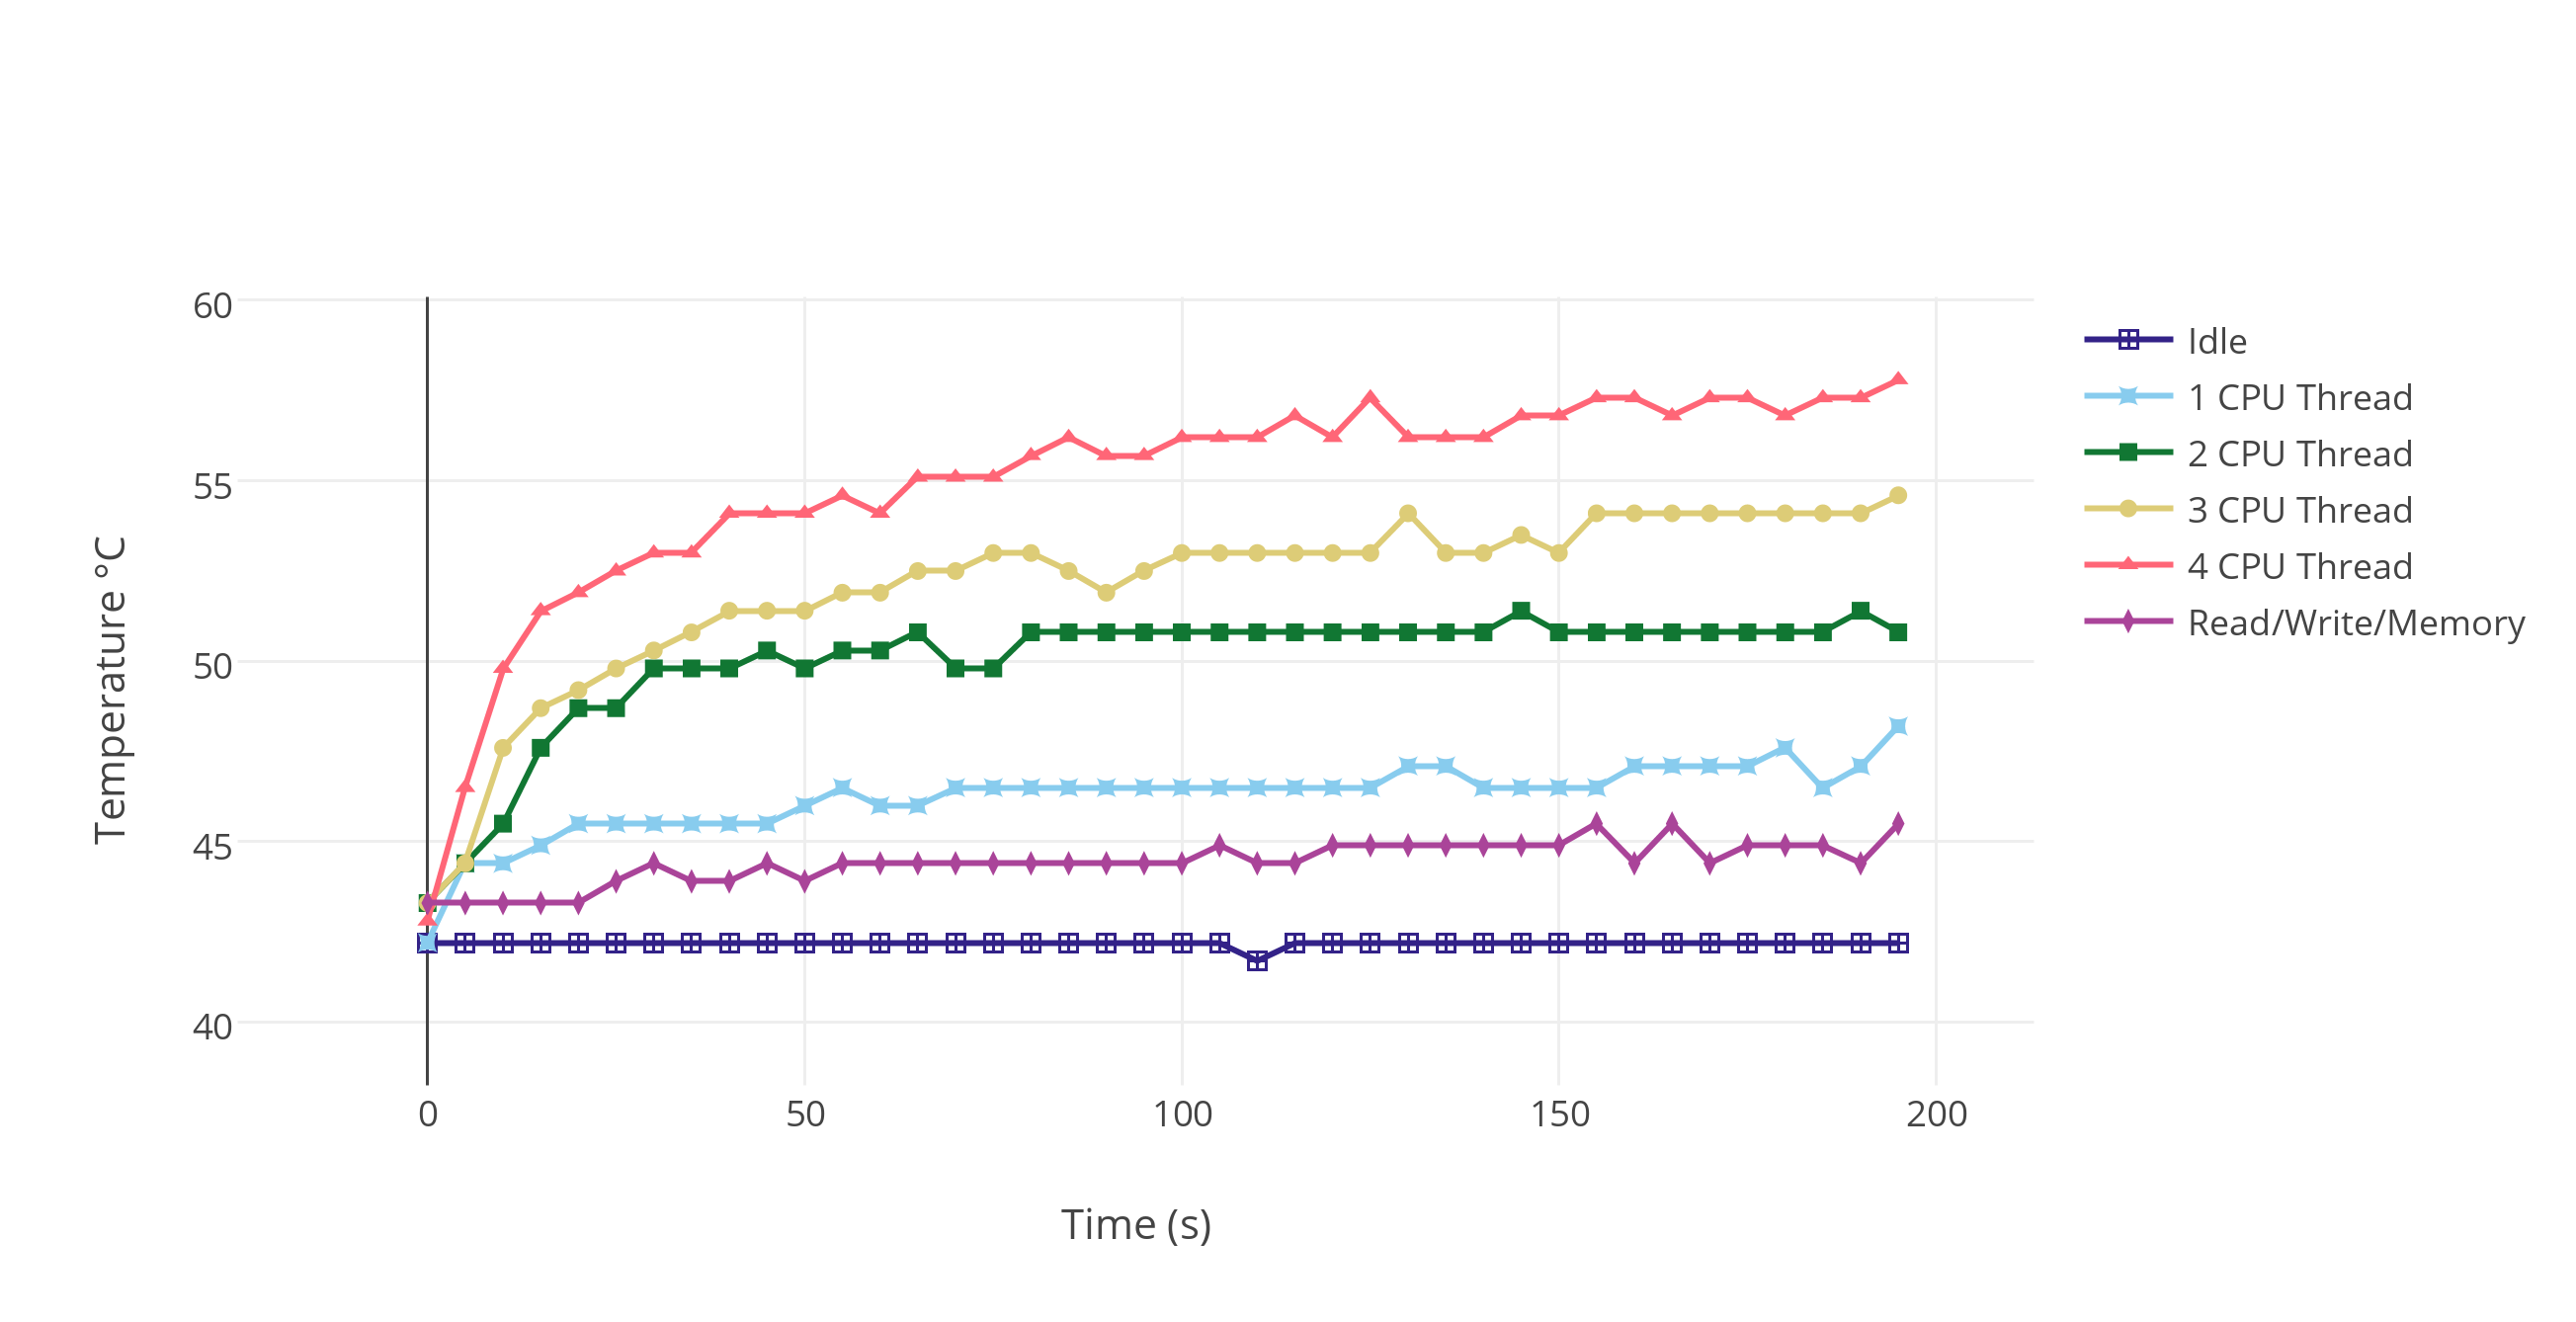
\includegraphics[scale=0.37]{Temperature_Test.png}
	\caption{Temperature Test}
	\label{fig:temp}
	
\end{figure}
When running a four thread CPU test the maximum temperature is 60 degrees Celsius and at idle the temperature is 42 degrees Celsius, see figure \ref{fig:temp}. Data centers require a temperature of around 26 degree Celsius \cite{temperature}. So if a lot of Raspberry Pi's are together some cooling is needed. This will require less cooling then a server. A server is still consuming 60 \% of its power and thereby producing a lot of heat. While Raspberry Pi's can be turned off and are better scalable. 


\subsection{RPi2 setup}\label{sec:setup}
In this setup we are going to make a Netflix kind of video stream service. \newline
\textbf{Dietpi} is the software used as operating system \cite{dietpi}. This is a diet version of Raspbian, the normal Raspberry Pi operating service. Raspbian is a diet version of Linux \cite{raspberry-pi}. This means that Dietpi only has the most necessary software to operate. By using Dietpi the memory usage for the operating system stays low. This low memory usage is important, because the creation of different video formats requires a lot of process and memory power. \newline
\textbf{NGINX}~\cite{nginx}: For the load balancing and streaming over HTTP NGINX is used. NGINX has a efficient algorithm to do HTTP load balancing. A RTMP module from Arut for NGINX is used to make a media streaming server over HTTP \cite{arut}. This is a efficient algorithm to transfer the HTTP with RTMP encapsulated data to the users. NGINX is optimized for ARM \cite{nginx}. This is the processor the RPi2 is using. Another reason to choose for NGINX and not for the Apache webserver is that it uses less memory. NGINX has a more efficient model than Apache, therefore it can handle more HTTP requests \cite{nginxvsapache}. Besides, for NGINX and Apache the most documentation available on how to do video streaming \cite{nginxvsapache}. \newline
\textbf{FFmpeg} is a cross-platform solution to record, convert and stream audio and video \cite{ffmpeg}. Using this software makes adaptive streaming and streaming in different formats possible. \newline
\textbf{JW Player}~\cite{jwplayer}: JW Player is a HTML5/flash embedded media player. It is a open source media player. JW player makes it possible to do some load balancing dependable on the bit rate that is coming from the video. It supports dynamic streaming, that consists of multiple single streams with the same content, all in a different quality from different streams \cite{jwplayer}. The Player uses server modules to stream the video to the client using the formats HTTP FLV or H264.\newline
\textbf{Cassandra} is a database that helps replicating data across multiple data centers \cite{cassandra}. In the case of this project there are videos stored by using Cassandra. The data can automatically be replicated across the nodes for fault-tolerance. Therefore, the data is still available when a node crashes.


\subsection{Raspberry Pi 2  testing}\label{sec:test}

In this testing section several test are done. In appendix \ref{sec:software} are the results and software configuration. The following test were executed: 
\begin{enumerate}[topsep=0pt,itemsep=-1ex,partopsep=1ex,parsep=1ex] 
	\item CPU test
	\item Iperf test
	\item RTMP stream test
	\item Video on demand test
	\item SMIL test
	\item File location test
\end{enumerate}

\subsubsection{CPU test}

The RPi2s are stress tested to make sure that they are operating correctly. For this the program stress for Linux is used to monitor its health \cite{stress}. Stress is a workload generator to test if the CPU, memory and I/O are working correctly. All three RPi2s are tested using this program and are working correctly. \newline
Another test is done with FFmpeg. FFmpeg needs a lot of CPU power to create new videos in different formats. To measure the CPU usage the top command of Linux was used, this measures the processor activity in real time \cite{top}. In this test a 230 MB 720p MPEG-4 (MP4 ) video has been converted into three different lower quality videos, this required 200 \% of the CPU power. The output is a 120p, 240p and 480p video file. At 200 \% CPU 2 cores are used out of the four to produce the video, this results in the fact that the RPi2 can only process two videos into different formats at the same time. The RPi2 has limited storage available, so they cannot store all the different video formats. This results in that the RPi2 needs to produce  these videos quickly to different formats, this can lead to difficulties.  \newline
If the videos are streamed by using NGINX they use not so much processor power. The CPU power that is needed for a single stream is about 2 \% and this barely increases when more clients are listening to it. To test the stream it is watched in a web browser and the CPU is measured using the Linux top command \cite{top}. 


\subsubsection{Iperf test}

The Internet speed is an important aspect in video streaming. According to Netflix there is 5.0 Megabits per second needed to stream one HD movie \cite{netflix}. During the ipref test the RPi2 has with a maximum connection of  94.2 Mbps~\cite{ipref}. This would result in the possibility for a RPi2 to stream about 18 HD videos at the same time. A simultaneous request of data by multiple streams reduces the bandwidth. So if many people do at the same time a request this can influence the connection of the RPi2. 

\subsubsection{RTMP stream test}

In this test a RTMP steam is tested. This test is done with Apache JMeter to see how many streams a RPi2 can handle~\cite{jmeter}. This test is done with a laptop and RPi2. First a test case is created in Apache JMeter then a RTMP video stream is started and a stream is checked in a web page in a web browser. The reason to check it inside a web browser is because Apache JMeter can only measure HTTP captures. The result of this test is that it can handle 25 users for streaming MPEG-4 (MP4 ) files over HTTP. If there are more users used the video might freeze, because there is too much latency. This becomes worse the more users there are this is a linear decrease. The RTMP stream used in this test streams the video only in 720p format. \newline Another test is by opening a media player like VLC were the RTMP stream address from the RPi2 is opened. If the RTMP stream with the 230 MB video of 49 minutes is opened  there can be seen that the video freezes, this is due to buffering problems. The cause of this is that the buffer length is too long.  \newline
The RTMP stream is streaming about 800 kbit/s for a small 230 MB movie. Theoretically this would mean that according to the formula max users=bandwidth/bit rate stream it will result in 118 users. This is with the Raspberry Pi 2 having a 100 Mbit connection. As been seen in the test before it might already freeze at 25 users. This latency is introduced by the client which has not enough buffer time. Another problem is a converter is used to convert a video to the RTMP stream, the use of a converter causes latency. \newline
If then a different stream is created with for example a audio file of 9 minutes there is no freezing with the VLC player. \newline To test it in the browser a JW player is embedded inside the web page. This browser stream can be maxed with the 118 users that are theoretically possible with the 800 kbit/s stream of the small movie. This is because the latency is not that high duo to the smaller screen used and the lower buffer length.
 

\subsubsection{Video on demand test}
For the video on demand (VOD) test a RTMP stream with FFmpeg has been created and NGINX was started to share the video. VLC was then opened on the laptop to see if there were any differences between VOD and a normal RTMP stream. The difference between VOD and RTMP is huge. With the use of video on demand the freezing was not visible. VOD is better equipped to load the stream then only RTMP. With only RTMP it is only possible to watch what is at that moment being played like normal television. RTMP does not adjust the bit stream depending on the quality needed, which is something VOD does.

\subsubsection{SMIL test}
By using the SMIL protocol it is possible to choose a different video streaming rate for the same file, for example 120p or 480p version of a movie. You now can choose the quality by yourself. This is something that for example Youtube does. With SMIL there is the possibility to switch the quality depending on the amount of data that can get over the network. During the test with Apache JMeter 100 connections were simulated watching the video. There are two scenarios one were the user can choose the quality by himself and one were it is done automatically. For the first scenario the user could choose between the 120p, 240p or 480p version of the 230 MB movie earlier used. The test is done by simulating only 120p, only 240p, only 480p or only 720p of the movie. When the 480p version is used freezing could be seen. With the other two this was a lot less. This results in the fact that when users select their own quality it is possible that some freezing can occur. When the quality was selected depending on the amount of data that a user can receive then there occurred no freezing. In apache JMeter it was also possible to see some latency when testing the streams. To make this test possible videos of different qualities have been created. These video versions were created by FFmpeg and were the 720p, 480p, 240p and 120p version of the 230 MB video. 

\subsubsection{File location test}
For file location and database a Cassandra database has been made. This data server is also used by Netflix to locate the movies. It turned out that it was possible to run Cassandra after a lot of configuration for the Raspberry Pi was done. To see if Cassandra was running the Cassandra query language shell was  opened on each RPi2. This was done by using the cqlsh command which is the command to start the cluster and its terminal. The output of the cqlsh command showed that it was connected to the cluster and the IP address of the RPi2. \newline
NGINX has a load balancing algorithm over HTTP. In this test it was possible to redirect the user to the right video by using this algorithm. 

\section{Discussion}

A small data center is built by using Raspberry Pi's. Small data centers are being used to avoid bottlenecks. Using microservers in data centers improves the scalability of the data center. Microservers such as the RPi2 can be used in these data centers. Small data centers with video streaming are used to get an elastic network, that can scale data bandwidth needed for video streaming. It is used to make faster adaptation of the video quality possible. By using it the user gets the best video quality without freezing. 

It turned out that it is possible to make a video streaming cluster with RPi2s. The RPi2 cloud has a low power consumption, but is not good for video streaming due to its limited bandwidth and CPU performance. In the research it was possible to analyze what happens with the video streams inside the cluster and to a test device like a laptop. This makes it possible to see what happens at the begin part of the network, so video stream algorithms can be improved.  

The RPi2 is placed inside a data center. The RPi2 is a lot smaller and there can be placed several of them inside a data center instead of a server. The RPi2 can save energy, because they can be turned on and off more scalable and they do not consume so much energy as a normal server. 

The setup of the RPi2 cloud consists of a operating system, a fault-tolerant database, a webserver, a video converter and a video player. The RPi2 has made load balancing possible with a webserver and media player in a browser. In order to stream a video to the user a RTMP message is encapsulated in HTTP for the web browser. 
The RPi2 can make videos of different qualities with a video converter. In tests it turned out that this video converter could only convert two videos at the same time. A stream is made by using a video converter and webserver. For the file location it is possible to set up a scalable fault tolerant database, so it is possible to locate the files even if one node fails.
The video streaming with Video on Demand or adaptive streaming has a good performance using this setup. In the future it is likely that devices with a ARM processor are used in a data center. The ARM processor has the possibilities to make it dedicated for a special task. 

Video streaming affected by various load balancing techniques. In the research several load balancing techniques were used. The webserver offers load balancing over adaptive streaming, this is used for video on demand (VOD). To redirect the user to the video HTTP load balancing is done with a webserver. In this research it turned out that RTMP streaming or VOD have differences in the availability. By using VOD the streaming goes better and the user experiences less freezing. SMIL can cause freezing when the user chooses the quality by himself, because its bitrate might not be sufficient for the quality demanded, causing freezing. When the computer does the change in quality there is less freezing. By using these different load balancing techniques the performance and the user experience changes. Improvements on those load balancing techniques were not possible due to time constraints, but these improvements can be possible in future research. 

\section{Conclusion}
Video streaming services have an increasing number of users, which causes an increase in the amount of network traffic and thus also in the amount of steaming problems. Small data centers decrease streaming problems, because of their elastic nature, which allows them to handle fluctuating video steaming bandwidth. We used RPi2s in small data centers to efficiently analyze video steaming. The analysis can be used to improve availability, user experience, and efficiency. Steaming servers operate only up to 20 \% of their total uptime, while still using 60 \% of their electricity needs. Compared to current steaming servers, RPi2s have a lower temperature because their electricity consumption is significantly lower. Nevertheless, RPi2s have a limited data bandwidth, which influences the capability of steaming and therefore affects user experiences. The CPUs of RPi2s have limited processing capabilities.  Specialized microprocessors like ARM can very likely be used in the future to improve those capabilities. To conclude, performance can be more efficiently analyzed by using RPi2 clusters.

\section{Future work}
New possibilities with faster USB and Ethernet interface. It is possible to create a gigabit connection over USB 2.0, this could double the connection speed, so twice the amount of videos can be streamed. This will make better video streaming possible and more users can be reached over HTTP. Work together with streaming services such as NGINX to further develop video streaming services hosted by ARM processors. In the future it would also be possible to run a Cassandra service for the RPi2 this will make the file location of video's possible in a cluster. Netflix is currently looking for a specialist in  Peer-to-Peer distribution for their videos \cite{netflix}.  Peer-to-Peer distribution can be interesting with Raspberry Pi. Besides this it might be interesting to investigate Peer-to-Peer distribution in general and for video streaming in specific, there can be done research into the technology and legal aspect of  Peer-to-Peer distribution. Apache JMeter is the tool to test HTTP streaming, but it would be more ideal to test only the RTMP stream for the RTMP test.  This turned out to be impossible with this testing tool. It is useful to test only the RTMP stream next time. It might be that a Raspberry Pi 2 can fit more easily inside a data center by using Power over Ethernet or by making a special motherboard and Raspberry Pi 2 modules instead of a whole device. 

\section{Acknowledgments}
This paper would not have been possible without the help of Nick Shot and MSc Björn Postema. A special thanks to Björn Postema from the Design and Analysis of Communication Systems group of the University of Twente, for his insight, good ideas and providing the necessary materials for doing this research.

\bibliographystyle{abbrvnat}
\bibliography{sigproc}  % sigproc.bib is the name of the Bibliography in this case
% You must have a proper ".bib" file
%  and remember to run:
% latex bibtex latex latex
% to resolve all references
%
% ACM needs 'a single self-contained file'!
%
%\vspace{50 mm}

%APPENDICES are optional

\clearpage
\appendix

\section{Cost structure}\label{sec:cost}
\begin{figure}[H]
	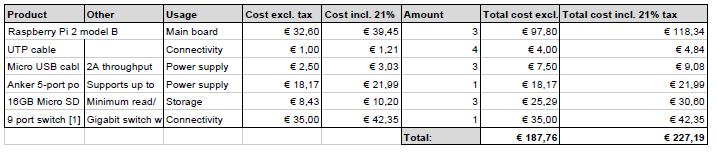
\includegraphics[scale=0.8]{cost_cluster.png}
	\label{fig:cost}
	\caption{Cost structure}
\end{figure}


\section{Software configuration and testing}\label{sec:software}

\subsection{Raspberry Pi 2}

\subsubsection{GitHub}
For more information about the project its possible to see the GitHub repository. Comments or questions about the code can be asked in the repository. \newline
The link is: \newline
\url{https://github.com/PaulVelthuis93/bachelorreferaat}

\end{document}